\chapter{Experimental Results} 
\label{ch:experimentalresults}

To evaluate the success of the composer, it seemed most appropriate to have a user experience study.  However, due to time constraints, development difficulties, and the nature of deployment, this has not yet happened.  Instead, the musical output of the tool will be judged from a music theory perspective.

\vspace{\baselineskip}

This section aims to determine whether or not the tool is able to correctly analyze a user created composition and provide appropriate details as how it can be fixed.  There are plans in the future to conduct a user study.  The questions that would be asked during that study are listed in the appendix.

\section{Musical Evaluation}
\label{sec:musicalevaluation}

To begin the musical evaluation, we will use the sample composition from Chapter 3.  It is displayed again below:

\begin{figure}[!htbp]
	\centering
	\caption{Notation Output}
	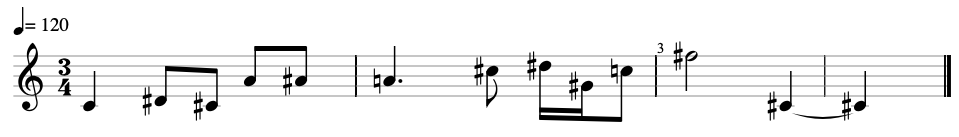
\includegraphics[scale=0.4]{images/notation.png}
\end{figure}

\pagebreak

\subsection{Areas of Analysis}
\label{subsec:areasofanalysis}

This melody will be analyzed for each of the rules that were outlined in Chapter 3.  When the analysis function is run on the sample melody, it returns the following data:

\begin{table}[!htbp]
	\centering
	\caption{Sample Melody Range}
	\begin{tabular}{|l|l|}
		\hline
		Range & A11 \\ \hline
	\end{tabular}
\end{table}

\begin{table}[!htbp]
	\centering
	\caption{Sample Melody Intervals}
	\begin{tabular}{|l|l|}
		\hline
		Interval 1 to 2 & A2 \\ \hline
		Interval 2 to 3 & M-2 \\ \hline
		Interval 3 to 4 & m6 \\ \hline
		Interval 4 to 5 & A1 \\ \hline
		Interval 5 to 6 & d1 \\ \hline
		Interval 6 to 7 & M3 \\ \hline
		Interval 7 to 8 & M2 \\ \hline
		Interval 8 to 9 & P-5 \\ \hline
		Interval 9 to 10 & d4 \\ \hline
		Interval 10 to 11 & A4 \\ \hline
		Interval 11 to 12 & P-11 \\ \hline
	\end{tabular}
\end{table}

\begin{table}[!htbp]
	\centering
	\caption{Sample Melody Key}
	\begin{tabular}{|l|l|}
		\hline
		Key & f\sh minor \\ \hline
		Correlation Coefficient & 0.5743 \\ \hline
	\end{tabular}
\end{table}

\subsubsection{Range}
\label{subsubsec:range}

The rule for range was that the distance between the highest and lowest pitch was not to exceed an octave and a half.  The highest note (F\sh 5) and lowest note (C4) have been circled.  The analysis program returned that the distance between these is an augmented eleventh.  This is exactly an octave and a half.  While it does not exceed the limit, it is close so this may be something that the user would want to address.

\begin{figure}[!htbp]
	\centering
	\caption{Range Analysis}
	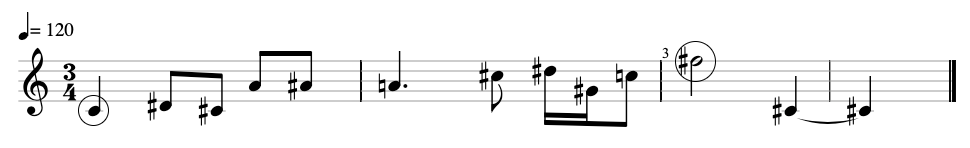
\includegraphics[scale=0.4]{images/range.png}
\end{figure}

\subsubsection{Contour}
\label{subsubsec:contour}

The rule for contour is that the ratio of steps to leaps should not exceed 3:1 and that leaps should be resolved by stepwise motion in the opposite direction as the leap.  The leaps have been surrounded by boxes.  The green boxes represent correctly resolved leaps and the red boxes indicate ones that were resolved incorrectly.

\vspace{\baselineskip}

The first box, while not adhering to any particular key, does resolve downwards with a major second after leaping an augmented second (minor third).  The next box, leaps up a minor sixth, but then, although by step, continues to move up an augmented first (minor second) when it should move downwards.  To fix this problem, the A\sh 4 could be changed to a G4.  The third and fourth box should be addressed similarly to the second box.

\vspace{\baselineskip}

The final box is a very good example of something that is entirely wrong.  The other boxes, even when resolved incorrectly, do not have as drastic of leaps as the last box.  Additionally, it is bad practice to have a leap as large as an eleventh.  To address this problem, the user should first resolve the leap from the C5 to the F\sh 5 with a move down to E.  Then, the user should potentially choose to end the melody on the F\sh 5 or bring the C\sh 4 up to a C\sh 5.  The F\sh 5 would be a better option, but the C\sh 5 is a possible choice.

\vspace{\baselineskip}

In this example, there are seven leaps and four steps.  This number of leaps far exceeds the targeted allowance.  This means that this melody would be very hard to sing since it is consistently jumping around.

\begin{figure}[!htbp]
	\centering
	\caption{Contour Analysis}
	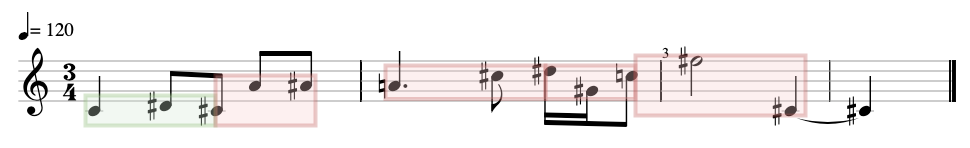
\includegraphics[scale=0.4]{images/contour.png}
\end{figure}

\subsubsection{Intervals}
\label{subsubsec:intervals}

The rule for intervals is that when there are leaps, these leaps should be of consonant intervals.  In this example, the steps and consonant leaps are marked in green and the dissonant leaps are marked in red.

\vspace{\baselineskip}

There are a number of issues with this melody in terms of intervals.  The biggest violation is that there are more dissonant intervals that consonant ones.  One of the easiest ways to fix this issue is related to the key.  By choosing notes that are outside of a particular key, the change for having dissonant intervals is greatly increased.

\vspace{\baselineskip}

Since the user is not required to understand keys, to address this interval problem, they should first address the key problem.  The key analysis feedback will help them to align the notes to a particular key.  After this step is completed, the analysis can be run again to see what problems still persist with the intervals.

\begin{figure}[!htbp]
	\centering
	\caption{Interval Analysis}
	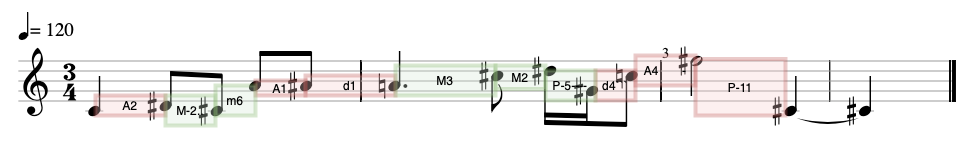
\includegraphics[scale=0.4]{images/intervals.png}
\end{figure}

\subsubsection{Key}
\label{subsubsec:key}

The reason that it was stated earlier that either the F\sh 5 or C\sh 5 is a possible choice to end the melody on is related to the fact that this melody is potentially in F\sh minor.  Both F\sh and C\sh are present in the F\sh minor chord, so they make possible ending pitches.  The F\sh is the better choice of the two since it is the tonic.

\vspace{\baselineskip}

The reason that it is potentially F\sh minor is due to the presence of a number of pitches that are not present in F\sh minor.  The analysis program lists the correlation as 0.5743.  This is not particularly high, but the fact that it is above half means that it is more likely F\sh minor.

\vspace{\baselineskip}

Seven out of the five notes belong in F\sh minor.  Those that belong in the key are marked in green and those that do not are marked in red.  Another potential reason for this melody being marked as F\sh minor is due to the highest note being F\sh and the final note being present in the F\sh minor triad.

\vspace{\baselineskip}

To improve the correlation and get this melody closer to F\sh minor, the C's should be sharp, the D's should be natural,  and the A's should be natural.  This would fix several of the problems related to dissonant intervals as well.

\begin{figure}[!htbp]
	\centering
	\caption{Key Analysis}
	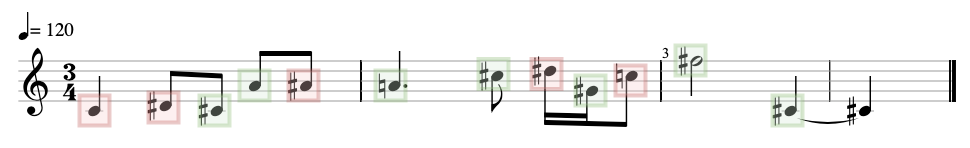
\includegraphics[scale=0.4]{images/key.png}
\end{figure}